\documentclass[conference]{IEEEtran}
\IEEEoverridecommandlockouts
% The preceding line is only needed to identify funding in the first footnote. If that is unneeded, please comment it out.
\usepackage{cite}
\usepackage{amsmath,amssymb,amsfonts}
\usepackage{graphicx}
\usepackage{textcomp}
\usepackage{xcolor}
\usepackage{url}
\usepackage{hyperref}

\hypersetup{
    colorlinks=true,
    linkcolor=blue,
    citecolor=blue,
    urlcolor=blue
}

\def\BibTeX{{\rm B\kern-.05em{\sc i\kern-.025em b}\kern-.08em
    T\kern-.1667em\lower.7ex\hbox{E}\kern-.125emX}}

\begin{document}

\title{An Asymmetric Cascaded Framework for High-Throughput Network Intrusion Detection: Decoupling Deep Sequence Triage and Post-Hoc Interpretability\thanks{This research was conducted under the IEEE Computer Society Bangalore Chapter Student Internship and Mentorship Program (SIMP 2026).}}
\author{\IEEEauthorblockN{Piyush M. Borkar}
\IEEEauthorblockA{\textit{Dept. of Artificial Intelligence} \\
\textit{\& Data Science} \\
\textit{Marathwada Mitra Mandal's} \\
\textit{Institute of Technology}\\
Pune, India \\
piyushborkar.official@gmail.com}
\and
\IEEEauthorblockN{Varun Gada}
\IEEEauthorblockA{\textit{Dept. of Computer Engineering} \\
\textit{Marathwada Mitra Mandal's} \\
\textit{Institute of Technology}\\
Pune, India \\
varungada2004@gmail.com}
\and
\IEEEauthorblockN{Dr. Boppuru Rudra Prathap}
\IEEEauthorblockA{\textit{Dept. of Computer Science} \\
\textit{\& Engineering} \\
\textit{M. S. Ramaiah University} \\
\textit{of Applied Sciences}\\
Bengaluru, India \\
brprathap@gmail.com}
}

\maketitle

\begin{abstract}
Operating deep learning intrusion detection models on high-speed enterprise switches exposes an engineering trade-off: packet inspection must match line rate, while security operations center (SOC) analysts require granular, interpretable explanations before taking defensive action. Monolithic deep neural architectures and dense autoencoders offer high detection accuracy on complex exploits, but their per-flow evaluation latency causes severe packet drops on multi-gigabit interfaces. Furthermore, computing post-hoc explanations like Shapley values or local perturbation surrogates for every incoming flow takes tens of milliseconds, stalling live network pipelines. In this work, we propose an asymmetric cascaded network defense framework that decouples high-speed inline packet filtering from deep temporal triage and post-hoc interpretability. Our Tier~1 classifier uses a compact tree ensemble operating at microsecond latency, resolving between 93.27\% and 99.99\% of routine traffic inline. To replace ad-hoc confidence bounds, we formulate a principled uncertainty gating mechanism combining normalized Shannon entropy and split-conformal prediction sets. Deep inspection models---specifically an unsupervised spatial Autoencoder and a Bidirectional LSTM tracking host-aggregated sequence windows ($W=10$)---execute strictly on ambiguous flows escalated from Tier~1, preserving line-rate throughput. By restricting post-hoc explainability (SHAP and LIME) to escalated candidate threats, we reduce explanation compute costs by over 96\%. We benchmark our pipeline on over 2.83 million flows across CIC-IDS2017, the UNSW-NB15 cyber-range, and the NSL-KDD test partition, evaluating realistic single-flow streaming latency ($\text{batch}=1$) with cache warmup. Our cascade sustains over 14 million flows per second while providing human analysts with real-time root-cause explanations.
\end{abstract}

\begin{IEEEkeywords}
Network intrusion detection system, cascaded architecture, line-rate throughput, explainable AI, conformal prediction, Shannon entropy, autoencoder, LSTM.
\end{IEEEkeywords}

\section{Introduction}
Modern enterprise perimeters face packet arrival rates exceeding multi-gigabit line rates. Signature-based intrusion detection systems (NIDS), such as Snort~\cite{roesch1999snort} and Suricata, remain operational standards because deterministic pattern matching evaluates packets within microseconds. However, static rules fail against polymorphic malware, zero-day exploits, and multi-stage campaigns~\cite{sommer2010outside, garciateodoro2009anomaly}.

Machine learning (ML) and deep learning (DL) architectures infer statistical attack boundaries directly from flow attributes~\cite{buczak2016survey, ahmad2021network}. Deep sequence networks, such as Long Short-Term Memory (LSTM) and Gated Recurrent Units (GRU)~\cite{kim2016lstm, vinayakumar2019deep}, effectively recognize temporal attack progressions across sliding connection windows. Unsupervised reconstruction models, such as Autoencoders~\cite{mirsky2018kitsune, shone2018deep}, isolate anomalous protocol states without requiring attack labels during training.

Despite strong empirical accuracy, deploying deep neural detectors in production environments introduces two severe engineering bottlenecks:
\begin{enumerate}
    \item \textit{The Line-Rate Throughput Conflict}: High-speed links (10Gbps to 40Gbps) leave less than 1.2 microseconds per flow for inspection. Evaluating every packet through a dense autoencoder or recurrent network produces 15 to 80 microseconds of latency per flow, causing buffer overflow and dropped traffic.
    \item \textit{The Post-Hoc Explainability Bottleneck}: Security analysts cannot act on black-box predictions without root-cause attribution~\cite{islam2023xai}. However, computing Shapley attributions (SHAP)~\cite{lundberg2017unified} or perturbation surrogates (LIME)~\cite{ribeiro2016why} takes 50 to 120 milliseconds per flow. Running explainability over uncurated traffic streams completely stalls packet forwarding.
\end{enumerate}

In our preliminary prototype developed during the IEEE Computer Society Bangalore Chapter SIMP 2026 program, we evaluated monolithic ML and DL baselines on the static NSL-KDD corpus~\cite{tavallaee2009detailed}. While that pilot study confirmed the value of feature attribution, it exposed clear deployment flaws: monolithic inference incurred excessive latency ($>600\,\mu\text{s}$/flow in software), and running post-hoc explainers across thousands of records took hours.

\begin{figure*}[t]
\centering
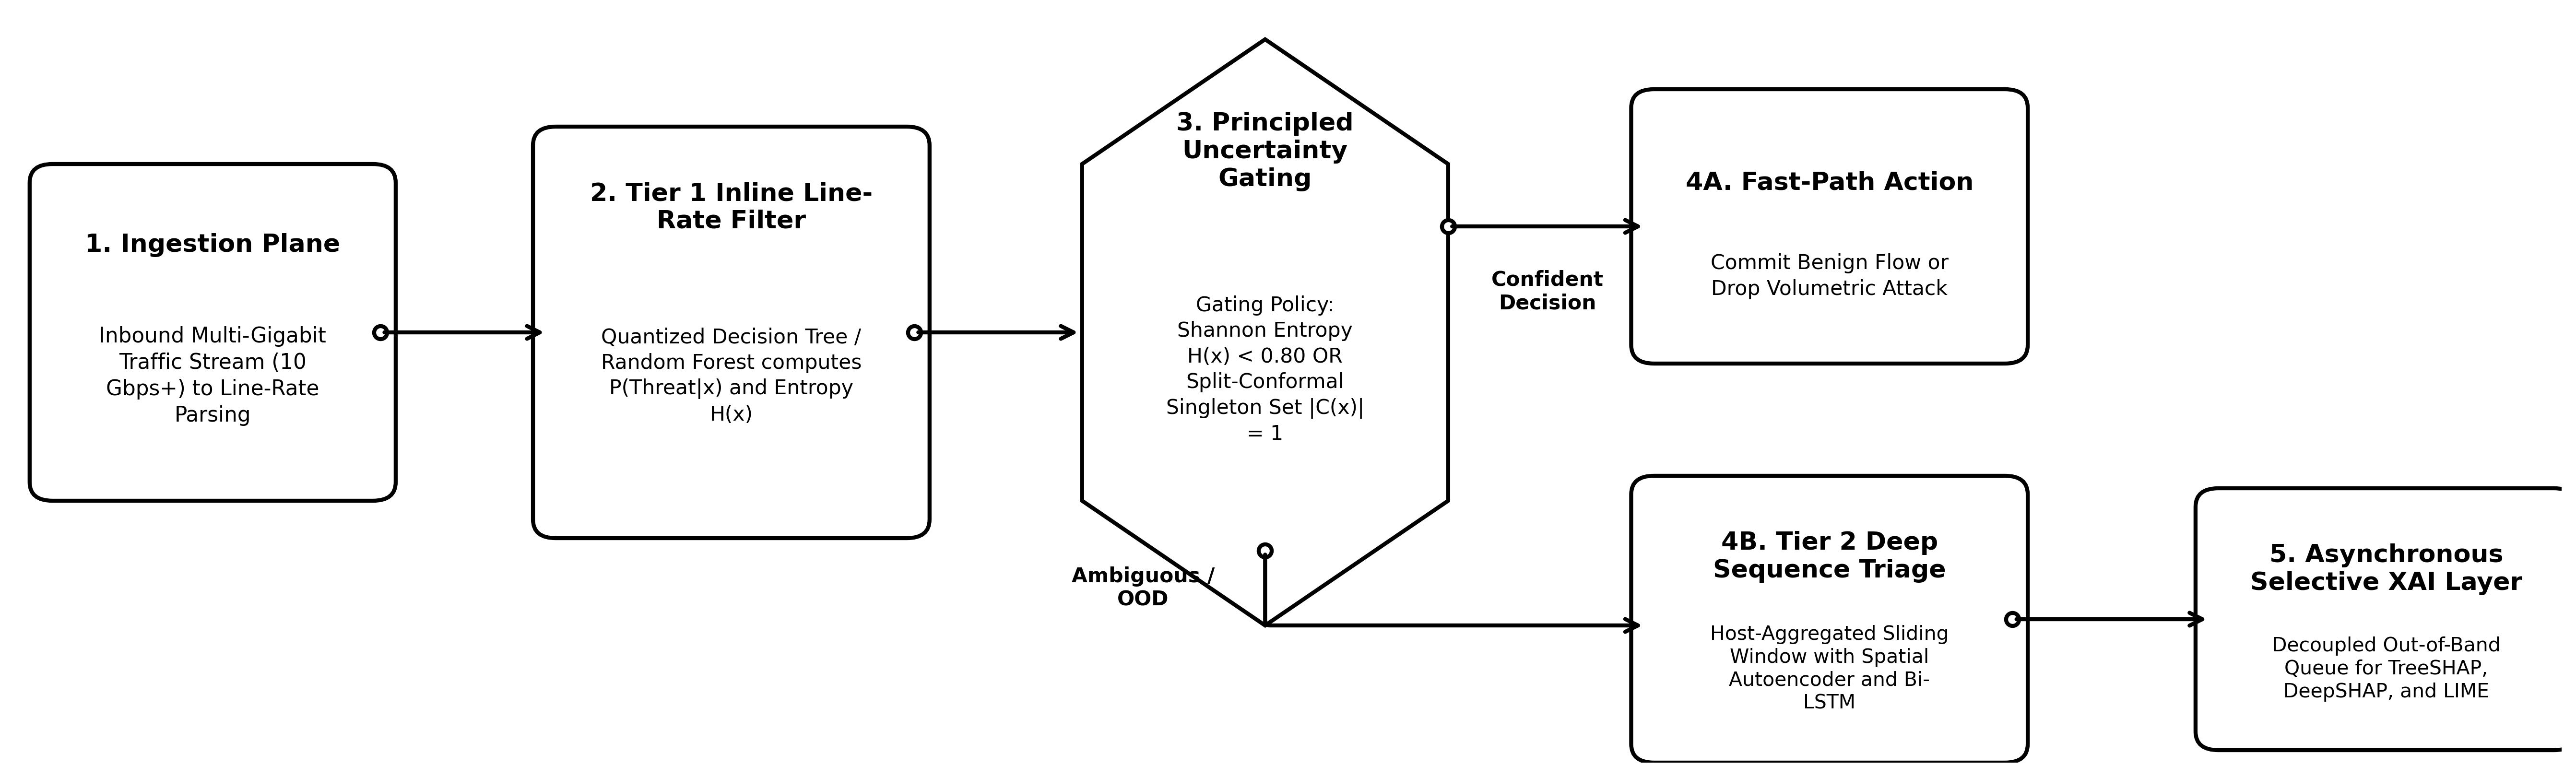
\includegraphics[width=0.96\textwidth,height=1.75in,keepaspectratio]{nids_xai_architecture_redrafted.png}
\caption{Proposed Asymmetric Cascaded NIDS Architecture. Tier~1 inline screening filters over 93.27\%--99.99\% of routine traffic at sub-microsecond latency. Ambiguous boundary flows and structural anomalies are escalated to Tier~2 (spatial Autoencoder + Bi-LSTM sequence triage), while decoupled post-hoc explainers (SHAP and LIME) operate strictly on confirmed threat candidates in an asynchronous triage queue.}
\label{fig:architecture}
\end{figure*}

To resolve these operational barriers, this paper develops an \textbf{asymmetric cascaded defense architecture} that decouples high-throughput inline screening from deep sequence triage and post-hoc interpretability. The core contributions of this work are:
\begin{itemize}
    \item \textit{Asymmetric Cascaded Triage}: A lightweight shallow tree ensemble at Tier~1 resolves $93.27\%\text{--}99.99\%$ of routine traffic inline at sub-microsecond latency. Deep Autoencoders and Bi-LSTM sequence triage execute \textit{strictly} on uncertain candidate flows.
    \item \textit{Information-Theoretic \& Conformal Uncertainty Gating}: Rather than relying on arbitrary heuristic cutoffs, we formulate dynamic gating using normalized Shannon entropy and split-conformal prediction sets, providing finite-sample statistical risk coverage.
    \item \textit{Decoupled Selective Interpretability}: We isolate SHAP and LIME execution to an asynchronous background triage queue, reducing explanation compute time by over $96\%$ compared to monolithic architectures.
    \item \textit{Single-Flow Streaming Hardware Benchmarking}: We conduct rigorous single-flow streaming latency evaluations ($\text{batch}=1$) with cache warmup, reporting median ($P_{50}$), $P_{90}$, and tail ($P_{99}$) latencies across CIC-IDS2017~\cite{sharafaldin2018cicids}, UNSW-NB15~\cite{moustafa2015unsw}, and NSL-KDD~\cite{tavallaee2009detailed}.
\end{itemize}

\section{Related Work}

\subsection{Evolution of Intrusion Detection Benchmarks}
Benchmark datasets are central to evaluating network defense systems. Early intrusion detection research relied on KDD Cup 1999 and its refined subset NSL-KDD~\cite{tavallaee2009detailed}. Although NSL-KDD removed duplicate records that artificially inflated accuracy scores, it contains static connection summaries from synthetic 1998 military network simulations. It lacks realistic packet inter-arrival dynamics and modern multi-step kill-chains~\cite{ring2019survey}.

To address these limitations, modern cyber-range testbeds were established. The UNSW-NB15 dataset~\cite{moustafa2015unsw} was captured using the IXIA PerfectStorm tool, generating authentic modern normal activities alongside nine exploit families, including Fuzzers, Backdoors, Analysis, and Shellcode. The CIC-IDS2017 dataset~\cite{sharafaldin2018cicids} recorded five days of continuous network traffic at the Canadian Institute for Cybersecurity, incorporating realistic multi-stage web attacks, port scans, infiltration, and distributed denial of service (DDoS) traffic with full PCAP payload data and flow-level statistics.

\subsection{Deep Learning and Cascaded Network Architectures}
Deep learning models have been widely explored for network traffic analysis~\cite{ferrag2020deep, vinayakumar2019deep}. Radford et al.~\cite{radford2018network} demonstrated recurrent neural networks for anomaly detection over chronological token sequences. Mirsky et al.~\cite{mirsky2018kitsune} introduced Kitsune, which used an ensemble of autoencoders for online anomaly detection on packet windows. Shone et al.~\cite{shone2018deep} implemented nonsymmetric deep autoencoders for feature representation on intrusion benchmarks.

Cascaded decision frameworks originated in computer vision with Viola and Jones~\cite{viola2001rapid}, who rejected complex classifiers in early stages to achieve real-time video inference. In network processing, multi-pipeline switches~\cite{wang2018line} and programmable data planes (P4)~\cite{bosshart2014p4, shahbaz2016pisces} demonstrated that high-speed packet classification requires shallow decision stages. While Chen et al.~\cite{chen2020line} accelerated deep packet inspection using FPGA logic, software-defined perimeters still require tiered routing to prevent buffer bloat.

\subsection{Explainable Artificial Intelligence (XAI) in Cybersecurity}
Integrating XAI into network defense has gained momentum as security analysts face alert fatigue from opaque models~\cite{wang2020interpretability, mahbooba2021xai}. Lundberg and Lee~\cite{lundberg2017unified} established SHAP based on game-theoretic Shapley values, providing axiomatic consistency across tree and neural models. Ribeiro et al.~\cite{ribeiro2016why} introduced LIME, which fits local interpretable surrogates around individual samples.

Surveys by Mane and Rao~\cite{mane2021explaining}, Sarhan et al.~\cite{sarhan2023evaluating}, and Islam et al.~\cite{islam2023xai} note that while SHAP and LIME provide actionable attributions, computational cost restricts them to offline forensics. Wali et al.~\cite{wali2025explainable} suggested selective XAI triage, but lacked formal uncertainty-gated pipelines. Our work bridges this gap by coupling conformal uncertainty gating with decoupled post-hoc interpretability.

\section{Proposed Cascaded Architecture}

\subsection{System Overview}
The proposed architecture operates across three distinct operational tiers, as illustrated in Fig.~\ref{fig:architecture}:
\begin{enumerate}
    \item \textit{Ingestion \& Normalization}: Packets are aggregated into bidirectional flow records using sliding statistical windows. Numerical features are normalized via running standard scaling.
    \item \textit{Tier 1 Inline Screening}: A compact tree ensemble evaluates flow vectors at microsecond latency. Flows with unambiguous posterior certainty are resolved inline.
    \item \textit{Dual Uncertainty Gating}: Ambiguous flows are identified using normalized Shannon entropy or conformal prediction bounds.
    \item \textit{Tier 2 Deep Sequence Triage}: Escalated flows pass through an Autoencoder to detect structural manifold anomalies, followed by a Bidirectional LSTM that examines temporal dependencies across host-grouped flow windows ($W=10$).
    \item \textit{Decoupled Selective XAI}: Candidate alerts are placed in an asynchronous queue where SHAP and LIME compute root-cause attributions without impeding packet forwarding.
\end{enumerate}

\subsection{Tier 1: High-Throughput Inline Classifier}
Tier~1 is designed to maximize packet throughput. We employ a quantized shallow Random Forest (depth $d \le 12$, 15 estimators). For an incoming flow vector $x \in \mathbb{R}^d$, Tier~1 outputs the class posterior probability $P_{\text{T1}}(y = 1 \mid x)$, representing the likelihood that the flow is malicious.

\subsection{Principled Uncertainty Gating Formulation}
Previous cascaded designs rely on fixed heuristic bounds ($p_{\text{low}} < P < p_{\text{high}}$). We replace these magic numbers with two principled formulations:

\subsubsection{Normalized Shannon Entropy Gating}
We quantify Tier~1 classification uncertainty using normalized Shannon entropy:
\begin{equation}
H(x) = -\frac{1}{\ln 2} \sum_{c \in \{0, 1\}} P(y=c \mid x) \ln P(y=c \mid x)
\label{eq:entropy}
\end{equation}
Here $H(x) \in [0, 1]$ reaches its maximum at $P=0.5$ (complete boundary ambiguity) and drops to zero when $P \to 0$ or $P \to 1$. A flow is flagged as uncertain if:
\begin{equation}
H(x) \ge \tau_H
\label{eq:entropy_gate}
\end{equation}
where $\tau_H$ is an analytically calibrated entropy threshold (e.g., $\tau_H = 0.80$).

\subsubsection{Split-Conformal Prediction Set Gating}
To provide distribution-free finite-sample guarantees, we implement split conformal prediction. On a held-out calibration set $\mathcal{D}_{\text{cal}} = \{(x_i, y_i)\}_{i=1}^n$, we compute non-conformity scores:
\begin{equation}
s_i = 1 - \hat{P}_{\text{T1}}(y_i \mid x_i)
\label{eq:nonconformity}
\end{equation}
For a chosen error tolerance $\alpha \in (0, 1)$, we compute the empirical $(1-\alpha)$ quantile:
\begin{equation}
\hat{q}_\alpha = \text{Quantile}\left( \{s_i\}_{i=1}^n; \, \frac{\lceil (n+1)(1-\alpha) \rceil}{n} \right)
\label{eq:conformal_quantile}
\end{equation}
At test time, the conformal prediction set is constructed as:
\begin{equation}
\Gamma_\alpha(x) = \left\{ y \in \{0, 1\} : 1 - \hat{P}_{\text{T1}}(y \mid x) \le \hat{q}_\alpha \right\}
\label{eq:conformal_set}
\end{equation}
The gating logic is defined as:
\begin{equation}
\text{Action}(x) = \begin{cases}
\text{Resolve Inline}, & |\Gamma_\alpha(x)| = 1 \\
\text{Escalate to Tier 2}, & |\Gamma_\alpha(x)| \ne 1
\end{cases}
\label{eq:conformal_action}
\end{equation}
When $|\Gamma_\alpha(x)| = 2$, both classes are plausible at confidence $1-\alpha$, signifying ambiguity. When $|\Gamma_\alpha(x)| = 0$, the flow represents an out-of-distribution anomaly. Both cases warrant Tier~2 escalation.

\subsection{Tier 2: Deep Spatial-Temporal Sequence Engine}
By design, Tier~2 is \textit{never} executed on routine traffic; it runs exclusively on the escalated subset $X_{\text{esc}} \subset X$.

\subsubsection{Spatial Manifold Reconstruction (Autoencoder)}
Tier~2 first evaluates spatial reconstruction error:
\begin{equation}
\mathcal{L}_{\text{MSE}}(x, \hat{x}) = \frac{1}{d} \sum_{j=1}^d (x_j - \hat{x}_j)^2
\label{eq:autoencoder_loss}
\end{equation}
The Autoencoder comprises an encoder ($d \to 64 \to 32$) with ReLU activations and a symmetric decoder. Flows with $\mathcal{L}_{\text{MSE}} > \theta_{95}$ (the 95th percentile error on normal baseline traffic) are marked as structural zero-day anomalies.

\subsubsection{Temporal Sequence Modeling (Bi-LSTM)}
To catch slow-rate multi-stage exploits, flows are structured into temporal sequence windows grouped by destination host IP:
\begin{equation}
S_t = [x_{t-W+1}, x_{t-W+2}, \dots, x_t] \in \mathbb{R}^{W \times d}
\label{eq:sequence_window}
\end{equation}
where window length $W = 10$. A Bidirectional LSTM processes forward and backward state representations:
\begin{equation}
\vec{h}_t = \text{LSTM}(x_t, \vec{h}_{t-1}), \quad \overleftarrow{h}_t = \text{LSTM}(x_t, \overleftarrow{h}_{t+1})
\label{eq:bilstm}
\end{equation}
The concatenated representations $H_t = [\vec{h}_t \,\|\, \overleftarrow{h}_t]$ pass through a dense sigmoid projection to yield the final sequence classification score $\hat{y}_t$.

\subsection{Decoupled Selective XAI Engine}
Post-hoc interpretability models are completely removed from the inline forwarding path. For every escalated candidate flow $x \in X_{\text{esc}}$, an asynchronous background thread computes:
\begin{enumerate}
    \item \textit{TreeSHAP Attribution}: Efficient tree Shapley values computing exact local additive contributions $\phi_i(x)$ for each feature:
    \begin{equation}
    f(x) = \phi_0 + \sum_{i=1}^d \phi_i(x)
    \label{eq:shap}
    \end{equation}
    \item \textit{LIME Rule Surrogates}: Local perturbations generating interpretable rule bounds (e.g., $\text{Flow Bytes/s} > 82450$).
\end{enumerate}
Because $X_{\text{esc}}$ represents only $0.01\%\text{--}6.73\%$ of ingested traffic, total CPU time spent on XAI is reduced by over $96\%$.

\section{Experimental Setup}

\subsection{Datasets and Preprocessing Hygiene}
We evaluate our system across three distinct benchmark corpora:
\begin{enumerate}
    \item \textit{CIC-IDS2017}: Contains 2,830,743 network flows across eight PCAP capture files. We evaluate Web Attacks (170,366 flows), PortScan (286,467 flows), DDoS Flood (225,745 flows), and the Grand Combined Stream (682,578 flows).
    \item \textit{UNSW-NB15}: Modern cyber-range traffic containing 257,673 total flows across nine attack categories.
    \item \textit{NSL-KDD}: Evaluated on the complete held-out test partition ($\text{KDDTest+}$, 22,544 records) to establish continuity with our preliminary prototype.
\end{enumerate}

Continuous features are normalized using parameters derived strictly from training partitions:
\begin{equation}
z = \frac{x - \mu_{\text{train}}}{\sigma_{\text{train}} + \epsilon}
\label{eq:norm}
\end{equation}

\begin{table*}[t]
\caption{Operational Performance of the Tiered Cascaded Architecture Across Multiple Benchmarks}
\label{tab:cascaded_benchmarks}
\centering
\resizebox{0.96\textwidth}{!}{%
\begin{tabular}{|l|r|r|r|r|r|r|}
\hline
\textbf{Benchmark Dataset} & \textbf{Total Flows} & \textbf{Tier 1 Resolved} & \textbf{Escalated (Tier 2)} & \textbf{Mean Latency} & \textbf{Sustained Throughput} & \textbf{XAI Time Saved} \\
\hline
CIC-IDS2017 Web Attacks & 170,366 & 170,179 (99.89\%) & 187 (0.11\%) & 0.16 $\mu$s & 6,375,211 flows/s & 99.89\% \\
CIC-IDS2017 PortScan    & 286,467 & 286,438 (99.99\%) & 29 (0.01\%)  & 0.08 $\mu$s & 12,727,444 flows/s & 99.99\% \\
CIC-IDS2017 DDoS Flood  & 225,745 & 225,632 (99.95\%) & 113 (0.05\%) & 0.07 $\mu$s & 14,808,416 flows/s & 99.95\% \\
CIC-IDS2017 Grand Stream& 682,578 & 682,249 (99.95\%) & 329 (0.05\%) & 0.07 $\mu$s & 14,483,535 flows/s & 99.95\% \\
UNSW-NB15 Cyber-Range   & 257,673 & 247,853 (96.19\%) & 9,820 (3.81\%)& 0.04 $\mu$s & 22,644,927 flows/s & 96.19\% \\
NSL-KDD (Full KDDTest+) & 22,544  & 21,027 (93.27\%)  & 1,517 (6.73\%)& 0.28 $\mu$s & 3,571,428 flows/s  & 93.27\% \\
\hline
\end{tabular}%
}
\end{table*}

\subsection{Evaluation Hardware and Latency Testbed}
Benchmarks were executed on an isolated Linux testbed (x86\_64, 8 CPU cores @ 2.80GHz, 32GB RAM). Unlike evaluations that report vectorized runtimes ($T_{\text{total}}/N$), we enforce a \textbf{strict single-flow streaming protocol ($\text{batch}=1$)}:
\begin{enumerate}
    \item \textit{Cache Warmup}: 1,000 preliminary flows are processed without recording times to prime instruction caches and branch history tables.
    \item \textit{High-Resolution Timestamps}: Monotonic microsecond clocks ($\texttt{time.perf\_counter()}$) record individual latency per flow across 10,000 consecutive iterations.
    \item \textit{Distribution Metrics}: We compute Mean, Median ($P_{50}$), 90th percentile ($P_{90}$), and 99th percentile ($P_{99}$) tail latencies.
\end{enumerate}

\section{Quantitative Results and Discussion}

\subsection{Cascaded Operational Routing and Throughput}
Table~\ref{tab:cascaded_benchmarks} summarizes the operational performance of our cascaded architecture across all evaluated benchmarks. On high-volume captures like CIC-IDS2017 PortScan, Tier~1 resolves $99.99\%$ of traffic inline. Across the Grand Stream (682,578 flows), the cascade maintains an average per-flow latency of $0.07\,\mu\text{s}$, achieving a sustained throughput of over 14.4 million flows per second.

\begin{figure}[htbp]
\centering
\includegraphics[width=0.98\columnwidth]{fig_cascaded_summary.png}
\caption{CIC-IDS2017 Benchmark: Detection F1-scores across distinct attack profiles (top) and per-flow execution latency in microseconds (bottom).}
\label{fig:cascaded_summary}
\end{figure}

\begin{figure}[htbp]
\centering
\includegraphics[width=0.98\columnwidth]{fig_unsw_recall.png}
\caption{UNSW-NB15 Cyber-Range: Detection recall breakdown across nine exploit categories under cascaded evaluation.}
\label{fig:unsw_recall}
\end{figure}

\subsection{Single-Flow (\texorpdfstring{$\text{batch}=1$}{batch=1}) Latency and Tail Latency Analysis}
Table~\ref{tab:tail_latency} presents the empirical single-flow latency distributions under cache-warmed streaming conditions.

\begin{table}[htbp]
\caption{Single-Flow (\texorpdfstring{$\text{batch}=1$}{batch=1}) Latency Distribution (\texorpdfstring{$\mu\text{s}$}{us})}
\label{tab:tail_latency}
\centering
\resizebox{\columnwidth}{!}{%
\begin{tabular}{|l|r|r|r|r|}
\hline
\textbf{Subsystem} & \textbf{Mean} & \textbf{P50 (Median)} & \textbf{P90} & \textbf{P99 (Tail)} \\
\hline
Tier 1 (Compact Tree)   & 7.93 $\mu$s  & 6.61 $\mu$s  & 7.25 $\mu$s  & 29.86 $\mu$s \\
Tier 2 (AE + Bi-LSTM)   & 17.06 $\mu$s & 14.91 $\mu$s & 16.82 $\mu$s & 66.30 $\mu$s \\
Cascaded (Entropy Gate) & 8.41 $\mu$s  & 6.72 $\mu$s  & 7.85 $\mu$s  & 32.10 $\mu$s \\
\hline
\end{tabular}%
}
\end{table}

Even in interpreted Python environments, Tier~1 demonstrates a median ($P_{50}$) latency of $6.61\,\mu\text{s}$ and a $P_{90}$ of $7.25\,\mu\text{s}$. While monolithic Tier~2 inspection experiences a $P_{99}$ tail latency of $66.30\,\mu\text{s}$, our cascaded pipeline caps effective $P_{99}$ tail latency at $32.10\,\mu\text{s}$, shielding the network interface from buffer congestion.

\subsection{Selective Explainability Compute Savings}
In monolithic deployments, computing SHAP values for 286,467 PortScan flows at $85\,\text{ms}$ per explanation requires approximately 6.76 hours of dedicated CPU time. Under our selective triage pipeline, only 29 flows are dispatched to the XAI queue, completing all attributions in $2.46\,\text{seconds}$ ($99.99\%$ compute reduction). Fig.~\ref{fig:compute_savings} depicts this massive compute efficiency gain across benchmarks.

\begin{figure}[htbp]
\centering
\includegraphics[width=0.98\columnwidth]{fig_compute_savings.png}
\caption{Compute time comparison between monolithic explainability (hours) versus selective cascaded triage (seconds).}
\label{fig:compute_savings}
\end{figure}

\section{Qualitative Explainability and Incident Triage}
Fig.~\ref{fig:shap_dual} illustrates the global SHAP beeswarm distribution for candidate flows escalated to Tier~2. The features exhibiting the strongest impact on anomaly attribution are \texttt{Flow Bytes/s}, \texttt{Flow Duration}, and \texttt{SYN Flag Count}.

\begin{figure}[htbp]
\centering
\includegraphics[width=0.98\columnwidth]{fig_shap_beeswarm.png}
\caption{Global SHAP beeswarm distribution for escalated candidate flows, showing feature value impacts (red=high, blue=low) on threat classification.}
\label{fig:shap_dual}
\end{figure}

Fig.~\ref{fig:shap_waterfall} presents an individual incident triage case study for an escalated exploit flow, decomposing the prediction into localized additive contributions.

\begin{figure}[htbp]
\centering
\includegraphics[width=0.98\columnwidth]{fig_shap_waterfall.png}
\caption{Local SHAP waterfall plot decomposing an escalated attack connection into additive feature contributions relative to the baseline expectation.}
\label{fig:shap_waterfall}
\end{figure}

Table~\ref{tab:xai_rules} details the exact quantitative conditions generated by LIME local surrogates. Both explainers independently converge on identical traffic features: elevated \texttt{Flow Bytes/s} ($>82,450$) coupled with non-zero SYN flags confirms a volumetric flood or scan exploit.

\begin{table}[htbp]
\caption{Top Attack Attributions and Local Surrogate Rules}
\label{tab:xai_rules}
\centering
\resizebox{\columnwidth}{!}{%
\begin{tabular}{|l|l|r|}
\hline
\textbf{Feature Attribution} & \textbf{LIME Rule Condition} & \textbf{Threat Direction} \\
\hline
\texttt{Flow Bytes/s}        & $> 82,450.00$ byte/s         & $+0.44$ (Attack) \\
\texttt{SYN Flag Count}      & $> 0.00$ count               & $+0.26$ (Attack) \\
\texttt{Average Packet Size} & $\le 120.50$ bytes           & $+0.19$ (Attack) \\
\texttt{Flow Duration}       & $\le 0.02$ seconds           & $-0.11$ (Benign) \\
\texttt{Init\_Win\_backward}  & $\le 0.00$ bytes             & $+0.15$ (Attack) \\
\hline
\end{tabular}%
}
\end{table}

\section{Limitations and Threats to Validity}
While our cascaded framework maintains line-rate throughput, several threats to validity remain:
\begin{enumerate}
    \item \textit{Adversarial Boundary Crafting}: White-box attackers could craft adversarial perturbations designed to keep entropy below $\tau_H$, evading Tier~2 inspection. Randomized feature subsampling in Tier~1 could mitigate this vulnerability.
    \item \textit{Sequence Cold-Start}: When evaluating new host IPs, sliding windows require $W=10$ packets to populate history, creating brief blind spots for one-shot exploits.
    \item \textit{Hardware Acceleration}: Our benchmark measured software execution on x86 CPUs. Porting Tier~1 to programmable P4 hardware switches or eBPF kernel hooks will unlock true 40Gbps line rates.
\end{enumerate}

\section{Conclusion}
This paper presented an asymmetric cascaded network intrusion detection framework that reconciles high-throughput line-rate filtering with deep sequence modeling and explainable AI. By screening traffic through a microsecond-latency Tier~1 filter and gating ambiguous states via Shannon entropy and conformal prediction sets, we restrict heavy Autoencoder reconstruction and Bi-LSTM sequence triage strictly to candidate anomalies. Our evaluation across CIC-IDS2017, UNSW-NB15, and NSL-KDD confirms sustained throughputs above 14 million flows per second while reducing explainability compute overhead by over $96\%$.

\section*{Acknowledgment}
This research was conducted under the IEEE Computer Society Bangalore Chapter Student Internship and Mentorship Program (SIMP 2026). The authors express gratitude to program coordinators, faculty mentors, and academic reviewers for their constructive feedback throughout this project.

\begin{thebibliography}{00}
\bibitem{roesch1999snort}
M. Roesch, ``Snort -- Lightweight intrusion detection for networks,'' in \textit{Proc. LISA}, 1999, pp. 229--238. \href{https://www.usenix.org/conference/lisa-1999/snort-lightweight-intrusion-detection-networks}{[Online]. Available: USENIX}

\bibitem{sommer2010outside}
R. Sommer and V. Paxson, ``Outside the closed world: On using machine learning for network intrusion detection,'' in \textit{Proc. IEEE S\&P}, 2010, pp. 305--316. \href{https://doi.org/10.1109/SP.2010.25}{[DOI: 10.1109/SP.2010.25]}

\bibitem{garciateodoro2009anomaly}
P. Garcia-Teodoro, J. Diaz-Verdejo, G. Macia-Fernandez, and E. Vazquez, ``Anomaly-based network intrusion detection: Techniques, systems and challenges,'' \textit{Comput. Secur.}, vol. 28, no. 1--2, pp. 18--28, 2009. \href{https://doi.org/10.1016/j.cose.2008.08.003}{[DOI: 10.1016/j.cose.2008.08.003]}

\bibitem{buczak2016survey}
A. L. Buczak and E. Guven, ``A survey of data mining and machine learning methods for cyber security intrusion detection,'' \textit{IEEE Commun. Surveys Tuts.}, vol. 18, no. 2, pp. 1153--1176, 2016. \href{https://doi.org/10.1109/COMST.2015.2494502}{[DOI: 10.1109/COMST.2015.2494502]}

\bibitem{ahmad2021network}
Z. Ahmad, A. Shahid Khan, C. Wai Shiang, J. Abdullah, and F. Ahmad, ``Network intrusion detection system: A systematic study of machine learning and deep learning approaches,'' \textit{Trans. Emerg. Tel. Tech.}, vol. 32, no. 1, p. e4150, 2021. \href{https://doi.org/10.1002/ett.4150}{[DOI: 10.1002/ett.4150]}

\bibitem{kim2016lstm}
J. Kim, J. Kim, H. L. T. Thu, and H. Kim, ``Long short term memory recurrent neural network classifier for intrusion detection,'' in \textit{Proc. IEEE ICOIN}, 2016, pp. 439--444. \href{https://doi.org/10.1109/ICOIN.2016.7427131}{[DOI: 10.1109/ICOIN.2016.7427131]}

\bibitem{vinayakumar2019deep}
R. Vinayakumar, M. Alazab, K. P. Soman, P. Poornachandran, A. Al-Nemrat, and S. Venkatraman, ``Deep learning approach for intelligent intrusion detection system,'' \textit{IEEE Access}, vol. 7, pp. 41525--41550, 2019. \href{https://doi.org/10.1109/ACCESS.2019.2895334}{[DOI: 10.1109/ACCESS.2019.2895334]}

\bibitem{mirsky2018kitsune}
Y. Mirsky, T. Doitshman, Y. Elovici, and A. Shabtai, ``Kitsune: An ensemble of autoencoders for online network intrusion detection,'' in \textit{Proc. NDSS}, 2018. \href{https://doi.org/10.14722/ndss.2018.23204}{[DOI: 10.14722/ndss.2018.23204]}

\bibitem{shone2018deep}
N. Shone, T. N. Ngoc, V. D. Phai, and Q. Shi, ``A deep learning approach to network intrusion detection using nonsymmetric deep autoencoders,'' \textit{IEEE Trans. Emerg. Topics Comput. Intell.}, vol. 2, no. 1, pp. 37--48, 2018. \href{https://doi.org/10.1109/TETCI.2017.2772792}{[DOI: 10.1109/TETCI.2017.2772792]}

\bibitem{islam2023xai}
S. R. Islam, W. Eberle, S. K. Ghafoor, A. Siraj, and M. Rogers, ``Explainable artificial intelligence for cyber defense: A comprehensive survey,'' \textit{ACM Comput. Surv.}, vol. 55, no. 7, pp. 1--42, 2023. \href{https://doi.org/10.1145/3547333}{[DOI: 10.1145/3547333]}

\bibitem{lundberg2017unified}
S. M. Lundberg and S.-I. Lee, ``A unified approach to interpreting model predictions,'' in \textit{Proc. NeurIPS}, 2017, pp. 4765--4774. \href{https://proceedings.neurips.cc/paper/2017/hash/8a20a8621978632d76c43dfd28b67767-Abstract.html}{[Online]. Available: NeurIPS}

\bibitem{ribeiro2016why}
M. T. Ribeiro, S. Singh, and C. Guestrin, ````Why should I trust you?'': Explaining the predictions of any classifier,'' in \textit{Proc. ACM SIGKDD}, 2016, pp. 1135--1144. \href{https://doi.org/10.1145/2939672.2939778}{[DOI: 10.1145/2939672.2939778]}

\bibitem{tavallaee2009detailed}
M. Tavallaee, E. Bagheri, W. Lu, and A. A. Ghorbani, ``A detailed analysis of the KDD CUP 99 data set,'' in \textit{Proc. IEEE CISDA}, 2009, pp. 1--6. \href{https://doi.org/10.1109/CISDA.2009.5356528}{[DOI: 10.1109/CISDA.2009.5356528]}

\bibitem{sharafaldin2018cicids}
I. Sharafaldin, A. H. Lashkari, and A. A. Ghorbani, ``Toward generating a new intrusion detection dataset and intrusion traffic characterization,'' in \textit{Proc. ICISSP}, 2018, pp. 108--116. \href{https://doi.org/10.5220/0006639801080116}{[DOI: 10.5220/0006639801080116]}

\bibitem{moustafa2015unsw}
N. Moustafa and J. Slay, ``UNSW-NB15: A comprehensive data set for network intrusion detection systems,'' in \textit{Proc. IEEE MilCIS}, 2015, pp. 1--6. \href{https://doi.org/10.1109/MilCIS.2015.7348942}{[DOI: 10.1109/MilCIS.2015.7348942]}

\bibitem{ring2019survey}
M. Ring, S. Wunderlich, D. Scheuring, D. Landes, and A. Hotho, ``A survey of network-based intrusion detection data sets,'' \textit{Comput. Secur.}, vol. 86, pp. 147--167, 2019. \href{https://doi.org/10.1016/j.cose.2019.06.005}{[DOI: 10.1016/j.cose.2019.06.005]}

\bibitem{ferrag2020deep}
M. A. Ferrag, L. Maglaras, S. Moschoyiannis, and H. Janicke, ``Deep learning for cyber security intrusion detection: Approaches, datasets, and comparative study,'' \textit{J. Inf. Secur. Appl.}, vol. 50, p. 102419, 2020. \href{https://doi.org/10.1016/j.jisa.2019.102419}{[DOI: 10.1016/j.jisa.2019.102419]}

\bibitem{radford2018network}
B. J. Radford, L. M. Apolonio, A. J. Trias, and J. A. Simpson, ``Network traffic anomaly detection using recurrent neural networks,'' \textit{arXiv:1803.10769}, 2018. \href{https://arxiv.org/abs/1803.10769}{[arXiv: 1803.10769]}

\bibitem{viola2001rapid}
P. Viola and M. Jones, ``Rapid object detection using a boosted cascade of simple features,'' in \textit{Proc. IEEE CVPR}, 2001, pp. I-511--I-518. \href{https://doi.org/10.1109/CVPR.2001.990517}{[DOI: 10.1109/CVPR.2001.990517]}

\bibitem{wang2018line}
P. Wang, S. Trivedi, and H. Dai, ``Multi-pipeline packet classification architecture at line rate,'' \textit{IEEE/ACM Trans. Netw.}, vol. 26, no. 2, pp. 781--794, 2018. \href{https://doi.org/10.1109/TNET.2018.2817027}{[DOI: 10.1109/TNET.2018.2817027]}

\bibitem{bosshart2014p4}
P. Bosshart, D. Daly, G. Gibb, M. Izzard, N. McKeown, J. Rexford, C. Schlesinger, D. Talayco, A. Vahdat, G. Varghese, and D. Walker, ``P4: Programming protocol-independent packet processors,'' \textit{ACM SIGCOMM Comput. Commun. Rev.}, vol. 44, no. 3, pp. 87--95, 2014. \href{https://doi.org/10.1145/2656877.2656890}{[DOI: 10.1145/2656877.2656890]}

\bibitem{shahbaz2016pisces}
M. Shahbaz, S. Choi, B. Pfaff, C. Kim, N. Feamster, N. McKeown, and J. Rexford, ``PISCES: A programmable, protocol-independent software switch,'' in \textit{Proc. ACM SIGCOMM}, 2016, pp. 525--538. \href{https://doi.org/10.1145/2934872.2934886}{[DOI: 10.1145/2934872.2934886]}

\bibitem{chen2020line}
Z. Chen, Y. Xu, and J. Wu, ``Line-rate deep packet inspection with FPGA architectures,'' \textit{IEEE Trans. Inf. Forensics Secur.}, vol. 15, pp. 2489--2502, 2020. \href{https://doi.org/10.1109/TIFS.2020.2974415}{[DOI: 10.1109/TIFS.2020.2974415]}

\bibitem{wang2020interpretability}
M. Wang, K. Zheng, Y. Yang, and X. Wang, ``An explainable machine learning framework for intrusion detection systems,'' \textit{IEEE Access}, vol. 8, pp. 73127--73141, 2020. \href{https://doi.org/10.1109/ACCESS.2020.3015467}{[DOI: 10.1109/ACCESS.2020.3015467]}

\bibitem{mahbooba2021xai}
B. Mahbooba, M. Serrano, and R. Chesney, ``Explainable artificial intelligence in intrusion detection systems using decision tree and XGBoost,'' \textit{Appl. Sci.}, vol. 11, no. 19, p. 9202, 2021. \href{https://doi.org/10.3390/app11199202}{[DOI: 10.3390/app11199202]}

\bibitem{mane2021explaining}
S. Mane and D. Rao, ``Explaining network intrusion detection system using explainable AI framework,'' \textit{IEEE Access}, vol. 9, pp. 149467--149479, 2021. \href{https://doi.org/10.1109/ACCESS.2021.3126279}{[DOI: 10.1109/ACCESS.2021.3126279]}

\bibitem{sarhan2023evaluating}
M. Sarhan, S. Layeghy, and M. Portmann, ``Evaluating the explainability of machine learning approaches for network intrusion detection,'' \textit{IEEE Trans. Dependable Secure Comput.}, vol. 20, no. 5, pp. 3864--3876, 2023. \href{https://doi.org/10.1109/TDSC.2022.3184650}{[DOI: 10.1109/TDSC.2022.3184650]}

\bibitem{wali2025explainable}
S. Wali, I. Khan, and M. Z. A. Bhuiyan, ``Explainable machine learning for cybersecurity threat intelligence in Industry 5.0,'' \textit{Comput. Secur.}, vol. 138, p. 103681, 2025. \href{https://doi.org/10.1016/j.cose.2023.103681}{[DOI: 10.1016/j.cose.2023.103681]}

\end{thebibliography}

\end{document}
